\chapter{The Sunayev-Zeldovich Effect}

\section{Atomic Physics}
The thermal \sze is one possible tracer. \sze is one type of spectral distortion in the CMB, one which refers to the inverse compton scattering of CMB photons off of hot electrons in the WHIM. In order for a spectral distortion to exist in the CMB, it must occur sufficiently late in the cosmological timeline that the radiation doesn't thermalise and regain a pure Planck spectrum (approximately $z < 2700$).

Compton Scattering is a form of inelastic scattering between light and free charged particles, such as electrons. There is a momentum transfer between the photon in the interaction, and the charged particle, and so the photon's wavelength changes as a result of the scattering. 

\begin{figure}[h!]
\centering
%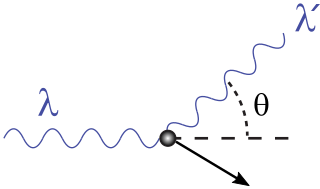
\includegraphics[scale=0.5]{/home/mitchell/Documents/masters/masters/thesis/Ver_2/figures/320px-Compton-scattering.png}
\feynmandiagram [horizontal=f2 to f3] {
  f1 [particle=\(e^{-}\)]-- [fermion] f2 -- [fermion] f3 -- [fermion] f4 [particle=\(e^{-}\)],
  f2  -- [photon] p1 [particle=\(\gamma\)],
  f3 -- [photon] p2 [particle=\(\gamma\)],
};
\label{fig:compton_scattering}
\caption{S-Channel Feynmann Diagram for Compton Scattering}
\end{figure}


It was first described in the context of X-rays interacting with electrons in atoms \citep{1923PhRv...21..483C}, and so regular Compton Scattering is taken to describe the interaction between a high energy photon, and a low energy particle. By applying principles of conservation of momentum, and conservation of energy,  the formula for the shift in wavelength as a result of this scattering is given by
\begin{equation}
	\Delta \lambda = \frac{h}{m_ec}\left(1-\cos\theta\right)
	\label{eqn:compton_shift}
\end{equation}
where $m_e$ is the mass of the electron, and $\theta$ is the angle between the incident and scattered trajectories. 

For the \sze however, the energies of the photons in question are much lower than the energies of the electrons involved, so the frequency shift is parametrised by something called the Compton $y$-parameter. The full expression for the Compton $y$-parameter is 
\begin{equation}
y = \int \frac{k_B T_e}{m_e c^2} n_e \sigma_T d \mathit{l}
\label{eqn:y_param}
\end{equation}
where $m_e c^2$, $k_B$, and $\sigma_T$ are the electron rest mass energy, Boltzmann constant, and Thompson Cross Section respectively. These are all well defined constants, and so have no effect on the integration. The $y$-parameter therefore amounts to the line-of-sight integration over $n_e T_e$, which are the electron gas density and temperature. The degeneracy between temperature and pressure can be broken in principle by obtaining measurements of one of the two quanties, which we in princple take from hydrodynamical simulations.

This $y$ parameter can be calculated in the CMB from frequency information. Starting from Kompaneets equation \citep{1957JETP....4..730K}, the time rate of change of the photon occupation number $\bar{n}$ due to Compton Scattering by non-relativistic, isotropic Maxwellian electron gas is given by a non-relativistic Fokker-Planck Equation \citep{1995ARA&A..33..541R}
\begin{equation}
\pdv{\bar{n}}{t} = \frac{kT}{mc} \frac{\sigma_T n_e}{x^2} \pdv{x} \left[ x^4 \left( \frac{T_e}{T} \pdv{\bar{n}}{x} + \bar{n} + \bar{n}^2 \right) \right]
\label{eq:fk_plnck}
\end{equation}
where $x = h \nu / k T$ is the non-dimensional frequency, $T$ is the temperature of the radiation, $n_e$ and $T_e$ are the number density and temperature of the electrons, and $\sigma_T$ is the Thompson cross section. Because $T_e >> T$, the first term in the parenthesis dominates, reducing the above to 
\begin{equation}
\pdv{\bar{n} }{t} = \frac{k T_e}{m c} \frac{\sigma_T n_e}{x^2} \pdv{x} \left(x^4 \pdv{\bar{n}}{x} \right)
\label{eq:reduced_fk_plnck}
\end{equation}
Since the incident radiation is only weakly scattered, an approximate solution to \ref{eq:reduced_fk_plnck} can be found by substituting the occupation number of a Planckian radiation field:
\begin{equation}
\bar{n_p}(x) = \frac{1}{e^x - 1} .
\label{eq:plnk_occupation_no}
\end{equation}
This makes the spectral form of the thermal \sze
\begin{equation}
g(x) = \frac{x^4 e^x}{(e^x-1)^2} \left[ \frac{x (e^x+1)}{e^x -1 } - 4 \right].
\end{equation}
\begin{figure}[h!]
\centering
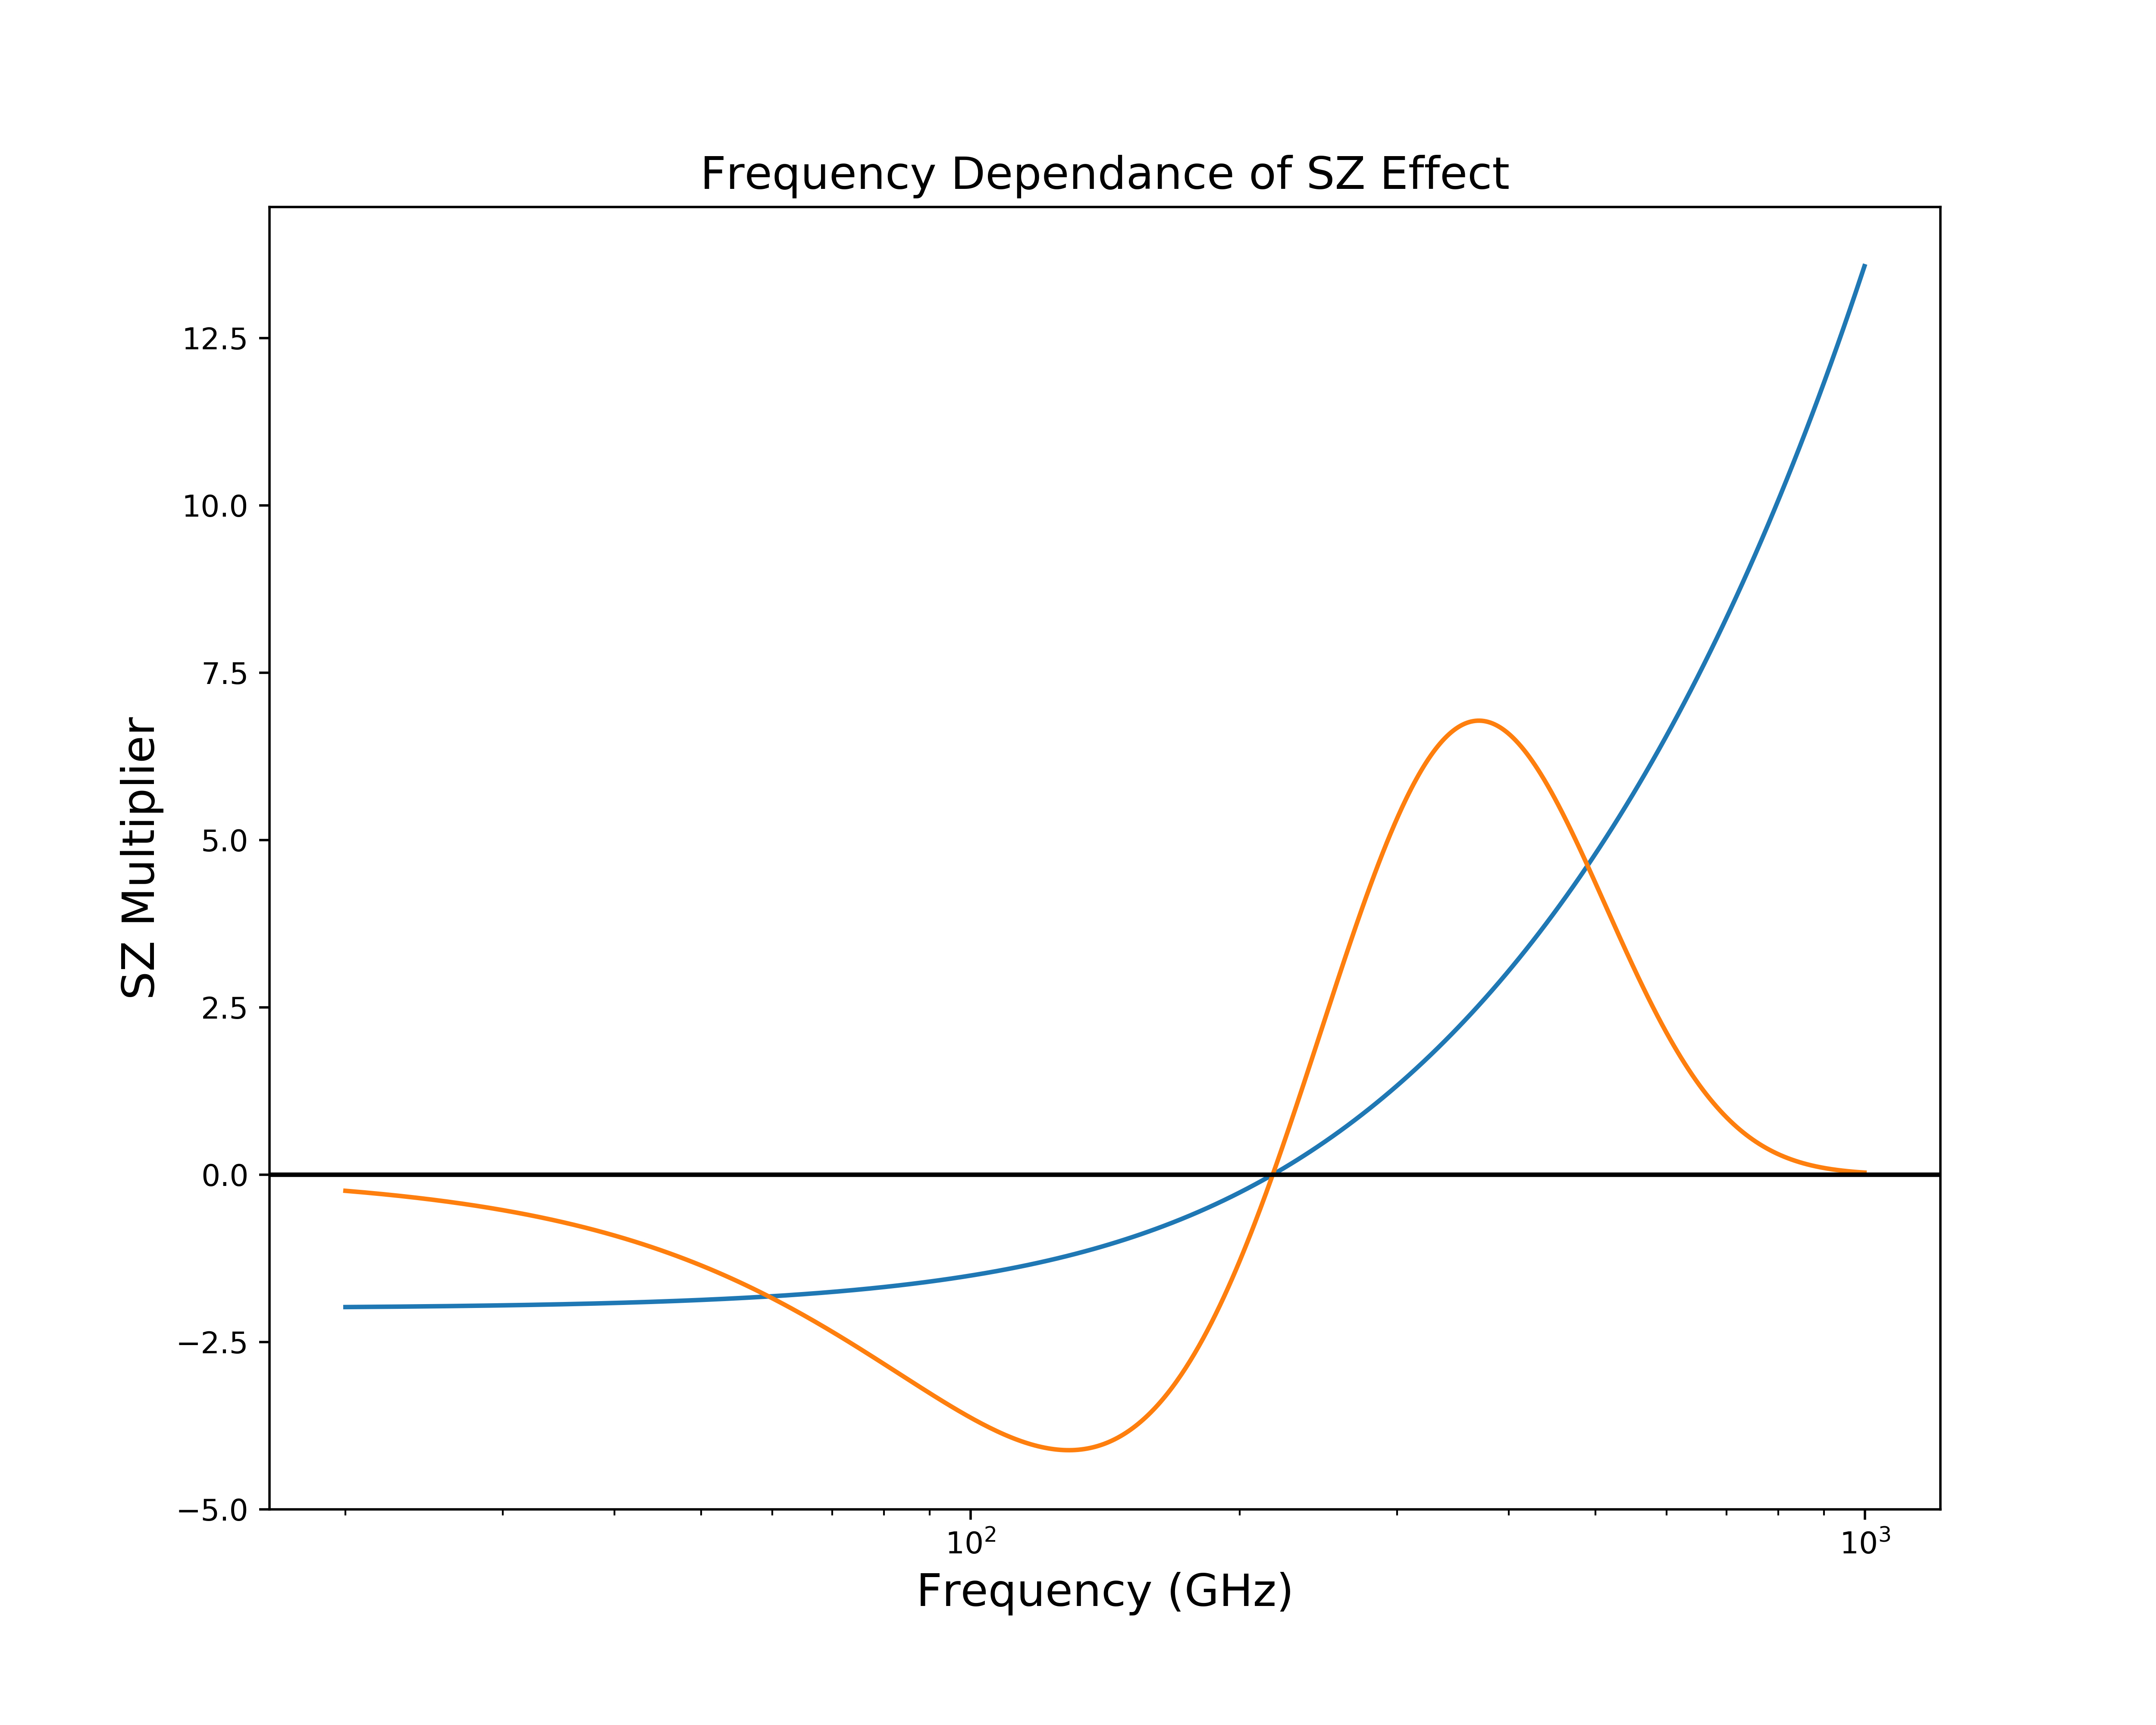
\includegraphics[scale=0.7]{/home/mitchell/Documents/masters/masters/thesis/Ver_2/figures/sz_freq.png}
\caption{\sze Intensity and Frequency Scaling Factors}
\label{fig:sz}
\end{figure}

Therefore, different frequency maps need to be scaled differently in order to account for the frequency of the photons incident on the gas. 


\section{CMB Signal}

The method for constructing a map of the \sze is given by variants on the 'Internal Linear Combination' (ILC) method \citep{2011MNRAS.410.2481R}. This method presumes very little about the form of the maps themselves, assuming that the maps can be written in the form 
\begin{equation}
\vec{x}(p) = \vec{a} s(p) + \vec{n}(p) 
\label{eq:ilc_1}
\end{equation}
where $\vec{x}$ is a vector of $N_{obs} $observations, $s(p)$ is a single map, $\vec{a}$ is a mixing vector, which does not depend on $p$ but is known, and $\vec{n}$ is some noise term, containing both instrument and astrophysical noise. It is also assumed that the maps are the same resolution.

The method then provides an estimator of the mean map, $\hat{s_{ILC}}(p)$ of the map $s$, by making a linear combination $\hat{s}(p) = \vec{w} \vec{x}(p)$:
\begin{equation}
\hat{s_{ILC}} = \frac{\vec{a^t} \hat{R^{-1}}}{\vec{a^t} \hat{R^{-1}} \vec{a}} \hat{x}
\end{equation}
where $\hat{R}$ is the covariance matrix of the observations. 

This method then allows for the map to essentially be linearly added together, in such a way the the variance is minimised, and so the resulting map is as close to the best fit as possible. 
\par One main advantage of the ILC component separation method is that it doesn't assume a model for the components that are not under direct consideration, they are simply collected in a catch-all nusiance term $\vec{n}(p)$. Unfortunately, if any of these components are correlated with the signals we are looking for, this method is unable to directly separate the signal from the noise without some \textit{a priori} knowledge of the components $a_i$.

An updated version of the algorithm, known as the modified internal linear combination algorithm (MILCA) \citep{2013A&A...558A.118H}, takes into account three changes to the above methodology. It accounts for localisation in pixel and spherical harmonic spaces to take into account and variations in spatial spectral laws. It also modifies the definition of the variance being minimised by an action of the covariance matix, to account for the possible correlation between noise and astrophyiscal sources.

Now, this technique can be applied to both the CMB as a whole, as well as the \sze specifically.  


The size of the anisotropy caused by the \sze can be determined from the number of clusters sampled from the observational beam. This number is highly dependant on the constraints on cluster evolution and their subsequent properties. The range of angular scales depends on the angular extent of the clusters, but ultimately sits within ranges of approximately $\SI{1}{\arcmin} - \SI{10}{\arcmin}$ , for a typical cluster with a radial extent of approximately $0.5 h_{-1} $Mpc, and a mass of $2\times 10^{15} M_\odot$. For this system, we expect that the size of the anisotropy to be roughly $\Delta T/T \approx 10^{-6} - 10^{-5}$ \citep{1995ARA&A..33..541R}. This makes sense, since the upper measure for the total Comptonisation of the CMB is only $4\times 10^{-3}$. However, it does pose an issue for detecting the WHIM, since the average density of a filament is so much lower than the density of a cluster. Given that the $y$ parameter is sensitive to the temperature of the gas and the number density, reducing the number density by a factor of $10^5-10^8$ and the gas temperature by $\sim 10^2$, will result in a corresponding reduction in the measured $y$ parameter. 

Given the signal-to-noise ratio expected for the thermal \sze of a single filament, many such filaments must be co-added, so as to drive the signal-to-noise to a detectable level. Initially outlined in \cite{2016MNRAS.457.2391C} for application to weak gravitational lensing maps, it was found that stacking $\sim 135 000$ pairs yielded a filament mass at $\sim 4.5 \sigma$ confidence. Further follow up using the Canada France Hawaii Telescope Lensing Survey (CFHTLenS), and the Sloan Digital Sky Survey's (SDSS) Luminous Red Galaxy (LRG) catalogue by \cite{2017MNRAS.468.2605E} detected the weak lensing signal from stacked filaments at 5$\sigma$ confidence.

Investigations by \cite{2014PhRvD..89b3508V}, \cite{2015JCAP...09..046M}, and \cite{2015JCAP...10..047H} established firmly that there is a correlation between weak gravitational lensing from CFHTLenS and tSZ signals from \emph{Planck} , which suggests that we can use tSZ in the same way as weak lensing, without having to be careful about the peculiarities assosciated with weak lensing, such as sufficiently nulling spherical components. This was further reinforced by \cite{2014JCAP...02..030H}, who reported a $6.2 \sigma$ correlation between the \emph{Planck}  lensing potential and the \emph{Planck}  tSZ map. 
